\documentclass{article}
\usepackage{fullpage}
\usepackage{graphicx}
\usepackage{tabularx}
\renewcommand{\arraystretch}{1.5}
\begin{document}
\title{Stakeholder Questions}
\author{Chiel Peters, Omar Pakker, Mary Gouseti, Cindy Berghuizen}
%\maketitle
\setlength\parindent{0pt}


\section{Questions}

\begin{tabularx}{\textwidth}{| l | X |}
  \hline
  \textbf{Stakeholder} & \textbf{1. State your stakeholder role. List the set of concerns you have that pertain to the architecture whose AD is being reviewed.} \\
  \hline
  EU Claim & Privacy of the users is guaranteed. Airline should handle situation appropriate. Transparancy is important, within the system, no airline should have more influence than another. \\
  \hline
  AirFrance-KLM & Be able to get in contact with the user. Have a reporting tool to see how the airline is doing. Enter flight information to combine with the rating. Other concerns are: costs and customer satisfaction. \\
  \hline
  Dutch Government & Representative of the Dutch government. Privacy and GreenIT are the concerns I have in this project. \\
  \hline
  Initiator & b. I am the initiator of this project. I want the project to be successful (become the nr1 site), profitable and online quickly. My main concern is the overall functionality of the system. \\
  \hline
\end{tabularx}

\begin{tabularx}{\textwidth}{| l | X |}
  \hline
  \textbf{Stakeholder} & \textbf{2. Find and record all places in the AD where your stakeholder role is listed as being covered.} \\
  \hline
  EU Claim & There is no list that the concerns are being covered. \\
  \hline
  AirFrance-KLM & There is no list that the concerns are being covered. \\
  \hline
  Dutch Government & Appendix A, p16, 1. Stakeholders, Stakeholder 3: Philipp Darkow. \\
  \hline
  Initiator & Appendix A, p16, 1. Stakeholders, Stakeholder 1: Peter Klijn. \\
  \hline
\end{tabularx}

\begin{tabularx}{\textwidth}{| l | X |}
  \hline
  \textbf{Stakeholder} & \textbf{3. Find and record all places in the AD where your concerns are listed as being addressed.} \\
  \hline
  EU Claim & Page 17: R1 \\
    & Page 19: Q4, Q5 \\
  \hline
  AirFrance-KLM & Page 16: F2 \\
    & Page 18: M3 \\
    & Functional Requirements: 5, 8, 9 \\
    & Page 19: Q1, Q2, Q3 \\
  \hline
  Dutch Government & Ch1, p6, GreenIT [R2] \\
    & Appendix A, p17, R2 \\
  \hline
  Initiator & Ch1, p6, Vendor lock-in [M2] \\
    & Appendix A, p16, F1 \\
    & Appendix A, p17, G1 \\
    & Appendix A, p17/18, M1 \\
    & Appendix A, p18, M2 \\
  \hline
\end{tabularx}

\begin{tabularx}{\textwidth}{| l | X |}
  \hline
  \textbf{Stakeholder} & \textbf{6. Record all concerns you have that are not listed as being covered in either the AD or any framework being used or that are listed in an unclear fashion. For each, state the impact of this omission or misunderstanding on project success.} \\
  \hline
  EU Claim & Privacy/security concerns are clearly stated in the document. Transparency can be found at Q4. Privacy not entirely if the admin can see al the data (not clear what the admin can / cannot do). \\
  \hline
  AirFrance-KLM & Everything is stated in the document. \\
  \hline
  Dutch Government & Privacy: system breaking. If the user's privacy can’t be guaranteed within the system, system development has to be halted till it does. In addition, by law user privacy has to be guaranteed unless the user agrees to sharing his information with people other than FlyWithUs. \\
  \hline
  Initiator & Nr 1 site: would be great to become the number one site but this does not impact the success of the project. \\
    & Profit: the project has to be able to be profitable. If it is not, the project will fail. (do something competitors do not do?) \\
    & Time till Deployment: the earlier the better but this does not prevent the project from succeeding. \\
  \hline
\end{tabularx}

\begin{tabularx}{\textwidth}{| l | X |}
  \hline
  \textbf{Stakeholder} & \textbf{7. For each of your concerns as a stakeholder, find and record the places in the AD where that concern is addressed (not just listed). Explain why you do or do not believe that the concern will be satisfied by the architecture.} \\
  \hline
  EU Claim & Privacy: Adressed on page 10 at Airline Rating Service Database on page 25 at seperate users table. This concerns will probably be satisfied by the architecture. The user database will be protected and located under dutch law. \\
    & Transparency: It is touched on page 15 at 'Filter and Store' and at 'Extract and Apply'. I am convinced it will be in the architecture but not in a very detailed way. \\
  \hline
  AirFrance-KLM & Usability: Page 6, "fast and easy to query" ; page 6: performance ; page 8 B2C application ; page 10: Airline Rating Service database ; Section 2.2;  page 18; functional requirements; page 19: Quality attribute Q2. \newline
  Since it is covered on a lot of difference places it will most probably be covered by the architecture. \\
    & Customer contact: Mentioned on page 19 and in the requirements, not convinced it will be in the architecture because that's the only mention found. \\
    & Cost: Page 4: vendor locking ; Page 6 Vendor locking ; It is not mentioned a lot, it probably isn't in the architecture but I'm not sure it should be. Cost more depends on what system/software you use instead of how the architecture looks (e.g. hadoop instead of storm). It could have been mentioned as a tradeoff for modifiability. \\
  \hline
  Dutch Government & GreenIT: Ch1, p6, GreenIT [R2] \newline
  I do not believe this is properly addressed because it is describing what GreenIT is without describing how these aspects are covered in the system. In addition, it does not give any grounded argumentation or facts for the choice of using a non-relational database. It seems to mostly rely on guesswork and a ‘gut-feeling’. \\
  \hline
  Initiator & Vendor lock-in: Ch1, p6, Vendor lock-in [M2] \newline
  While they say that by using an own implementation we prevent vendor lock-in, there is no word on how expensive this would be. Is this cheaper than using Hadoop? Is Hadoop really a vendor lock-in (ie. No alternatives or replacements possible once we use Hadoop?). What happened with the ‘Other distributed’ and ‘Undistributed’ options? \\
  \hline
\end{tabularx}

\begin{tabularx}{\textwidth}{| l | X |}
  \hline
  \textbf{Stakeholder} & \textbf{8. Find and record the place in the AD that prioritizes the concerns. Explain why you do or do not agree with it.} \\
  \hline
  All & There is no prioritization of the concerns. Some are mentioned in a way that they "must" or "should" be implemented, which may indicate a prioritization. The document in general lays a high focus on how the data is handled which gives a priority to performance and scalability. It is quite logical they lay a focus on this point because it is one of the biggest concerns overal and it may have a large effect on the architecture. \\
  \hline
\end{tabularx}

\begin{tabularx}{\textwidth}{| l | X |}
  \hline
  \textbf{Stakeholder} & \textbf{9. Record important stakeholders that you are aware of that are not listed and whose concerns are not represented in the AD.} \\
  \hline
  All & All the stakeholders are listed. \\
  \hline
\end{tabularx}

\begin{tabularx}{\textwidth}{| l | X |}
  \hline
  \textbf{Stakeholder} & \textbf{10. State how you know that the architecture satisfies the concerns of the missing stakeholders and where this information can be found in the AD.} \\
  \hline
  All & There are no missing stakeholders. \\
  \hline
\end{tabularx}


\newpage

\section{Scenarios}

\begin{tabularx}{\textwidth}{| l | X |}
  \hline
  \textbf{Scenario} & B2B - B2C decoupling \\
  \hline
  \textbf{Attribute} & Availability \\
  \hline
  \textbf{Environment} & Normal Operations \\
  \hline
  \textbf{Stimulus} & B2B or B2C failure \\
  \hline
  \textbf{Response} & Failure of either one does not influence the other. \\
  \hline
    &
    \begin{tabular}[t]{ | @{}| p{4cm} | l | l | l | l | @{} | }
      \hline
      \textbf{Architectural Decision} & \textbf{Sensitivity} & \textbf{Tradeoff} & \textbf{Risk} & \textbf{Non-risk} \\
      \hline
      Decoupling & S1 & T1 & & \\
      \hline
      Different API & S1 & T2 & & N1 \\
      \hline
    \end{tabular}
    \\
    &  T1: performance B2B vs performance B2C. \newline
    T2: redundant code (modifiability/maintainability) vs availability. \newline
    N1: Keeping the API as one still creates one point of failure for both B2B and B2C. \newline
    S1: If they are in the same server and the server goes down, B2C and B2B will both go down. \\
  \hline
  \textbf{Reasoning} & Decoupling ensures, together with the different API, that if one the B2B or B2C module goes down, the other won't. \\
  \hline
  \textbf{Architecture Diagram} & The red API crashes. \\
   & 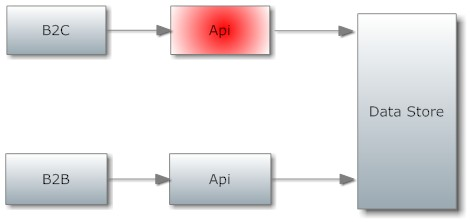
\includegraphics[width=300px]{scenario1} \\
  \hline
\end{tabularx}

\begin{tabularx}{\textwidth}{| l | X |}
  \hline
  \textbf{Scenario} & Peak load on the analytics module \\
  \hline
  \textbf{Attribute} & Performance \\
  \hline
  \textbf{Environment} & Normal Operations \\
  \hline
  \textbf{Stimulus} & Recalculating ratings/reviews \\
  \hline
  \textbf{Response} & B2B latency <10 sec. \\
  \hline
    &
    \begin{tabular}[t]{ | @{}| p{4cm} | l | l | l | l | @{} | }
      \hline
      \textbf{Architectural Decision} & \textbf{Sensitivity} & \textbf{Tradeoff} & \textbf{Risk} & \textbf{Non-risk} \\
      \hline
      Recalculate 1/2 times a day \newline (Implicit) & & & R1 & \\
      \hline
      B2B accesses analytics directly \newline (Implicit) & & T1 & & \\
      \hline
    \end{tabular}
    \\
    & R1: Creates peakload, leads to bad availability. \newline
    T1: Custom searches but there is a direct connect so if it fails of peak load, it is not available; Custom search vs peak load \\
  \hline
  \textbf{Reasoning} & Recalculating creates a massive peakload which may therefore cause an overload which may lead to an undesirable response time. When the B2B performs a custom search, it will not receive an answer in time. \\
  \hline
  \textbf{Architecture Diagram} & Analytics module overloaded. \\
   & 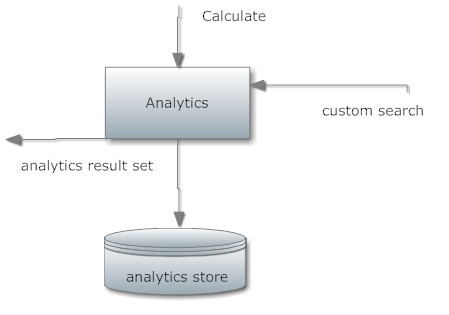
\includegraphics[width=300px]{scenario2} \\
  \hline
\end{tabularx}

\begin{tabularx}{\textwidth}{| l | X |}
  \hline
  \textbf{Scenario} & Review Privacy \\
  \hline
  \textbf{Attribute} & Privacy \\
  \hline
  \textbf{Environment} & Normal Operations \\
  \hline
  \textbf{Stimulus} & User writes a review \\
  \hline
  \textbf{Response} & Anonymous review \\
  \hline
    &
    \begin{tabular}[t]{ | @{}| p{4cm} | l | l | l | l | @{} | }
      \hline
      \textbf{Architectural Decision} & \textbf{Sensitivity} & \textbf{Tradeoff} & \textbf{Risk} & \textbf{Non-risk} \\
      \hline
      Logged In & & & R1 & \\
      \hline
    \end{tabular}
    \\
    & R1: Review is not anonymous. \\
  \hline
  \textbf{Reasoning} & No where in the document is stated that a review will be shown anonymous or how anonimity of reviews is guaranteed. \\
  \hline
  \textbf{Architecture Diagram} & Anyone can see review details. \\
   & 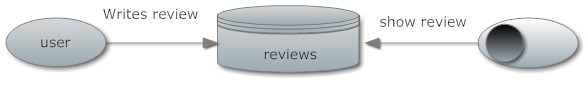
\includegraphics[width=300px]{scenario3} \\
  \hline
\end{tabularx}

\begin{tabularx}{\textwidth}{| l | X |}
  \hline
  \textbf{Scenario} & Big Data \\
  \hline
  \textbf{Attribute} & Performance, Availability \\
  \hline
  \textbf{Environment} & Normal Operations \\
  \hline
  \textbf{Stimulus} & Big Data input \\
  \hline
  \textbf{Response} & Handle all input without any loss of data. \\
  \hline
    &
    \begin{tabular}[t]{ | @{}| p{4cm} | l | l | l | l | @{} | }
      \hline
      \textbf{Architectural Decision} & \textbf{Sensitivity} & \textbf{Tradeoff} & \textbf{Risk} & \textbf{Non-risk} \\
      \hline
      ETL Adapters & & & & N1 \\
      \hline
      ETL Approaches & S1 & & & \\
      \hline
      Pipeline Structure & & & R1 & \\
      \hline
    \end{tabular}
    \\
    & S1: If it is Big data the system can not handle the input and a choke point will occur in the pipe model. \newline
    N1: Easily extendable, interdependent on eachother. \newline
    R1: Filter and store, Extract and Apply handle all reviews sequentially. \\
  \hline
  \textbf{Reasoning} & Because of the pipeline structure and the assumption the data is not regarded as big data the system won't be able to process more external sources when they become big data. \\
  \hline
  \textbf{Architecture Diagram} & <INSERT GRAPHIC> \\
  \hline
\end{tabularx}



% TABLE SCHEMATICS. (handy for copy/pasting in additional tables ;) )
%Questions table
\begin{tabularx}{\textwidth}{| l | X |}
  \hline
  \textbf{Stakeholder} & \textbf{<question>} \\
  \hline
  EU Claim & <answer> \\
  \hline
  AirFrance-KLM & <answer> \\
  \hline
  Dutch Government & <answer> \\
  \hline
  Initiator & <answer> \\
  \hline
\end{tabularx}

%Scenarios table
\begin{tabularx}{\textwidth}{| l | X |}
  \hline
  \textbf{Scenario} & <text> \\
  \hline
  \textbf{Attribute} & <text> \\
  \hline
  \textbf{Environment} & <text> \\
  \hline
  \textbf{Stimulus} & <text> \\
  \hline
  \textbf{Response} & <text> \\
  \hline
    &
    \begin{tabular}[t]{ | @{}| p{4cm} | l | l | l | l | @{} | }
      \hline
      \textbf{Architectural Decision} & \textbf{Sensitivity} & \textbf{Tradeoff} & \textbf{Risk} & \textbf{Non-risk} \\
      \hline
    \end{tabular}
    \\
    & <text> \\
  \hline
  \textbf{Reasoning} & <text> \\
  \hline
  \textbf{Architecture Diagram} & <text> \\
  \hline
\end{tabularx}



\end{document}